\section{System Architecture}

\begin{figure}[h]
\centering
  % Requires \usepackage{graphicx}
  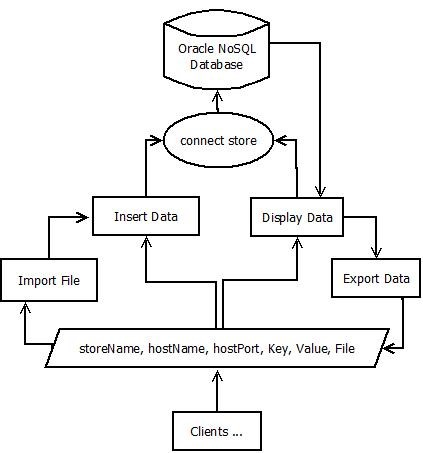
\includegraphics[width=14cm,height=13cm]{Fig10.jpg}\\
  \caption{System Architecture} \label{System Architecture}
\end{figure}

Brief summary of the software architecture is described below in the form of following UML Diagrams :
\begin{enumerate}
  \item State transition diagram
  \item Sequence diagram
  \item Collaboration diagram
  \item Package diagram
  \item Component diagram
  \item Deployment diagram
\end{enumerate}

\subsubsection{State transition diagram}
\hspace*{0.7in} A state machine diagram models the behavior of a single object specifying the sequence of an event that an object goes through during lifetime in response to events. Elements used in state diagram are Initial state, state, transition, history state, final state, signals etc. The most common purpose for which you will use state machines is to model the lifetime of an object, especially instance of classes, use cases and the system as a whole.
\\
\begin{figure}[h]
\centering
  % Requires \usepackage{graphicx}
  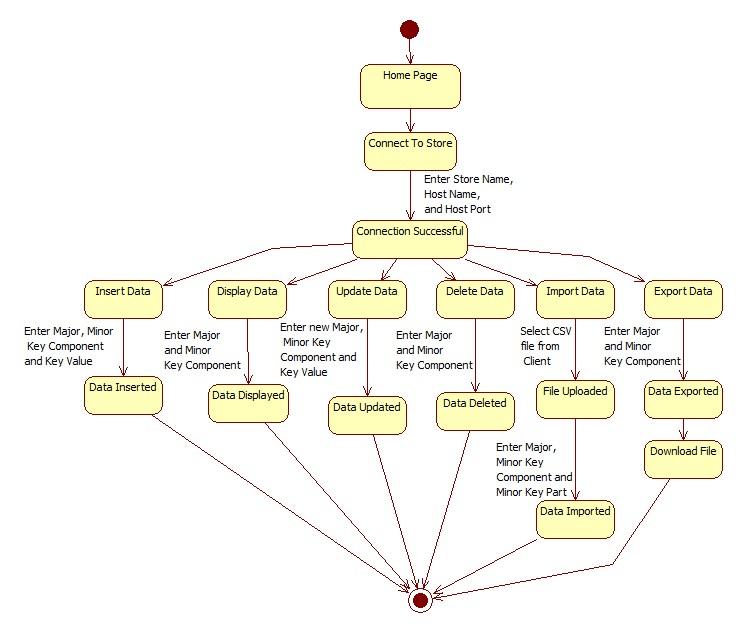
\includegraphics[width=13cm,height=10.5cm]{Fig11.jpg}\\
  \caption{State Transition For User}
  \label{State Transition For User}
\end{figure}

\newpage
\begin{itemize}
  \item GUI based  System :
\end{itemize}

\begin{figure}[h]
\centering
  % Requires \usepackage{graphicx}
  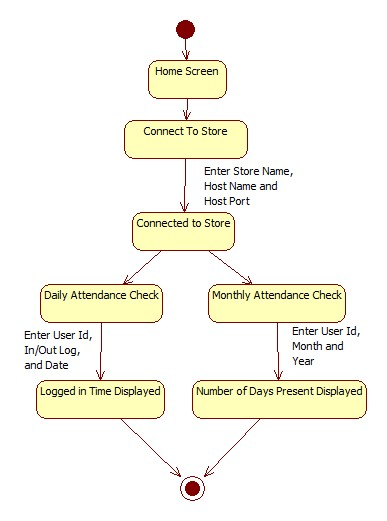
\includegraphics[width=8cm,height=13cm]{Fig12.jpg}\\
  \caption{Attendance check  System}
  \label{Attendance check  System}
\end{figure}

\subsubsection{Sequence diagram}
\hspace*{0.7in} A sequence diagram in Unified Modelling Language (UML) is a kind of interaction diagram that shows how processes operate with one another and in what order. It is a construct of a Message Sequence Chart. A sequence diagram shows, as parallel vertical lines (lifelines), different processes or objects that live simultaneously, and, as horizontal arrows, the messages exchanged between them, in the order in which they occur. This allows the specification of simple runtime scenarios in a graphical manner.
\begin{figure}[h]
\centering
  % Requires \usepackage{graphicx}
  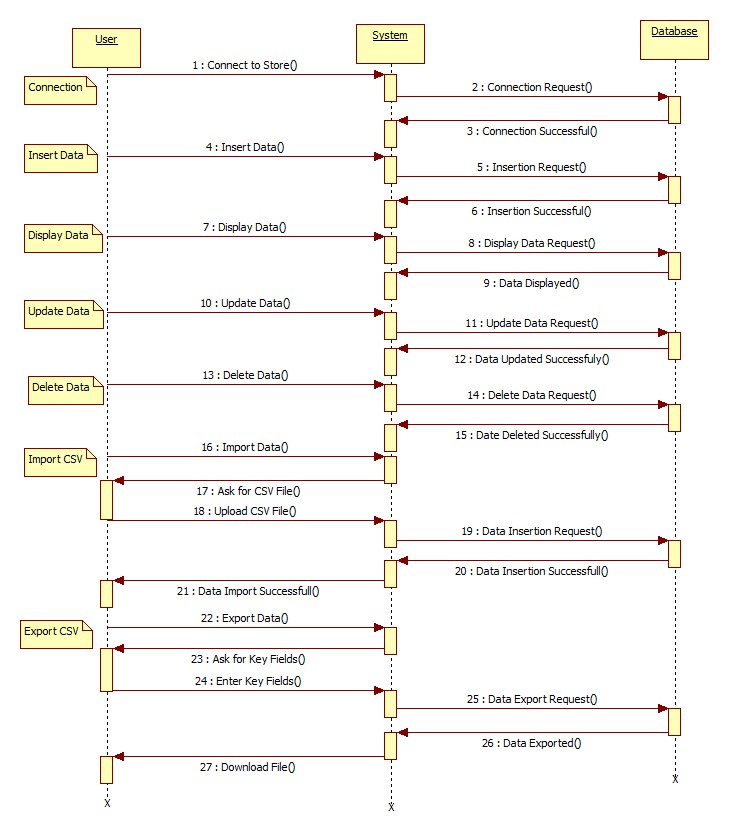
\includegraphics[width=15cm,height=15cm]{Fig13.jpg}\\
  \caption{Sequence Diagram}
  \label{Sequence Diagram}
\end{figure}

\newpage
\begin{itemize}
  \item GUI based  System :
\end{itemize}
\begin{figure}[h]
\centering
  % Requires \usepackage{graphicx}
  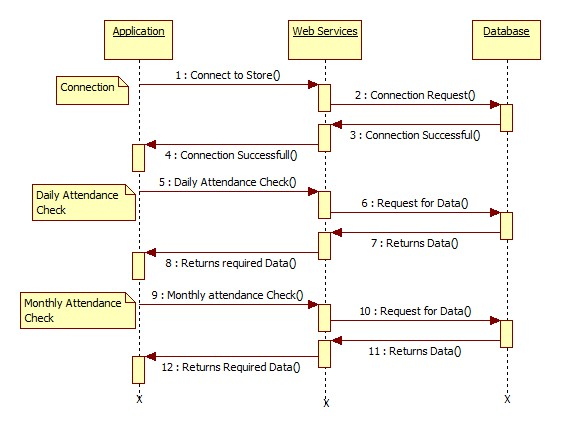
\includegraphics[width=13cm,height=8cm]{Fig14.jpg}\\
  \caption{Attendance check  System}
  \label{Attendance check  System}
\end{figure}

\newpage
\subsubsection{Collaboration diagram}
\hspace*{0.7in} A collaboration diagram describes interactions among objects in terms of sequenced messages. Collaboration diagrams represent a combination of information taken from class, sequence, and use case diagrams describing both the static structure and dynamic behavior of a system.

\begin{figure}[h]
\centering
  % Requires \usepackage{graphicx}
  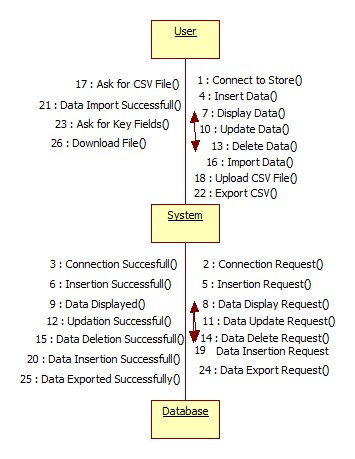
\includegraphics[width=7cm,height=8cm]{Fig15.jpg}\\
  \caption{Collaboration Diagram}
  \label{Collaboration Diagram}
\end{figure}
\newpage
\begin{itemize}
  \item GUI based  System :
\end{itemize}

\begin{figure}[h]
\centering
  % Requires \usepackage{graphicx}
  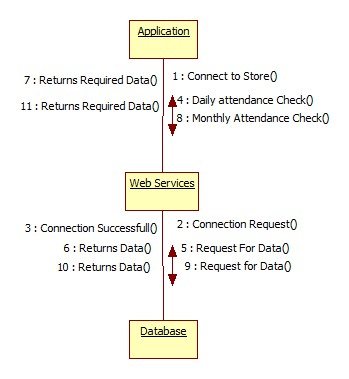
\includegraphics[width=6cm,height=8cm]{Fig16.jpg}\\
  \caption{Attendance check  System}
  \label{Attendance check  System}
\end{figure}

\subsubsection{Package diagram}
\hspace*{0.7in} Package is general purpose mechanism for organizing elements into groups. Every package must have a name that distinguishes it from other packages. Package name must be unique within its enclosing package .A name is a textual string .That name alone is known is known as simple name. A path name is package name prefixed by name of package lives.
\\
\begin{figure}[h]
\centering
  % Requires \usepackage{graphicx}
  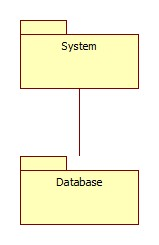
\includegraphics[width=4cm,height=5cm]{Fig17.jpg}\\
  \caption{Package Diagram}
  \label{Package Diagram}
\end{figure}
\\
\newpage
\begin{itemize}
  \item GUI based  System :
\end{itemize}
\begin{figure}[h]
\centering
  % Requires \usepackage{graphicx}
  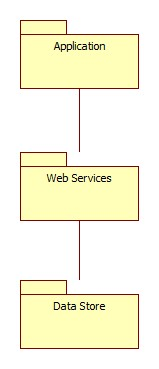
\includegraphics[width=5cm,height=8cm]{Fig18.jpg}\\
  \caption{Attendance check  System}
  \label{Attendance check  System}
\end{figure}

\subsubsection{Deployment Diagram}
\hspace*{0.7in} Deployment diagram represents the deployment view of a system. It is related to the component diagram. Because the components are deployed using the deployment diagrams. A deployment diagram consists of nodes. Nodes are nothing but physical hardware used to deploy the application.

\begin{figure}[h]
\centering
  % Requires \usepackage{graphicx}
  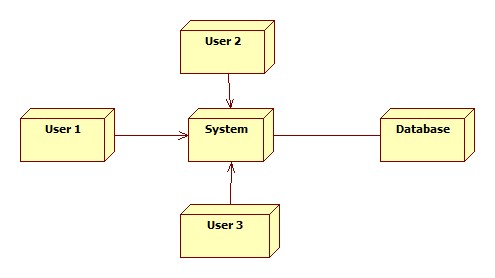
\includegraphics[width=8cm,height=7cm]{Fig19.jpg}\\
  \caption{Deployment Diagram}
  \label{Deployment Diagram}
\end{figure}
\newpage
\begin{itemize}
  \item GUI based  System :
\end{itemize}

\begin{figure}[h]
\centering
  % Requires \usepackage{graphicx}
  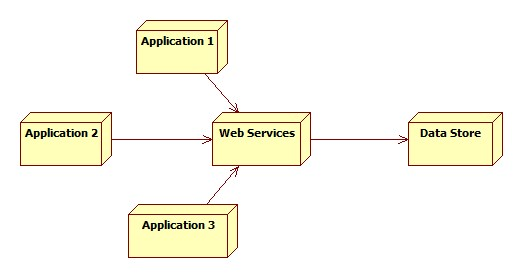
\includegraphics[width=8cm,height=7cm]{Fig20.jpg}\\
  \caption{Attendance check  System}
  \label{Attendance check  System}
\end{figure}
